\chapter{استراتيجية التصنيع والكيمياء الخضراء}\label{ch:g12:synthesis-strategy}

صُنع المسكّن نفسه، الإيبوبروفين، بطريقتين. فالطريق الأقدم
يمر بست خطوات، ومن كل مئة كيلوغرام من المواد الأولية
التي يشتريها ينتهي ستون نفايات. والأحدث يمر بثلاث
خطوات، ويحفظ كل \omterm{def:g7:atoms-and-molecules:atom}{ذرة} يشتريها تقريبًا. وكلاهما يعطي المسحوق الأبيض
نفسه في القرص؛ والفرق في التخطيط. فالكيميائي الذي يخطط
لتصنيع يطرح أربعة أسئلة: كيف يُسرع، وكيف يحصل على الكثير، وكيف
لا يمس إلا الجزء الصحيح من \omterm{def:g7:atoms-and-molecules:molecule}{الجزيء}، وكيف يقلل الهدر.

\begin{recall}
التصنيع: التفاعل، والفصل، والتنقية، والتعرف؛ ومردوده
(\cref{ch:g10:synthesis-yield}). الأسهم المنحنية، \omterm{def:g12:curly-arrows:categories}{والاستبدال}،
والإضافة، \omterm{def:g12:curly-arrows:categories}{والحذف} (\cref{ch:g12:curly-arrows}). \omterm{def:g12:catalysis:catalyst}{والحفّاز} يسرّع
التفاعل دون أن يُستهلك (\cref{ch:g12:catalysis}). \omterm{def:g12:equilibrium:non-total}{والتفاعل غير
التام} يتوقف عند $Q = K$؛ وفائض من \omterm{def:g7:chemical-reactions:reactant}{متفاعل}، أو
نزع \omterm{def:g7:chemical-reactions:reactant}{ناتج}، يدفعه أبعد (\cref{ch:g12:equilibrium}).
\end{recall}

\begin{omfigure}
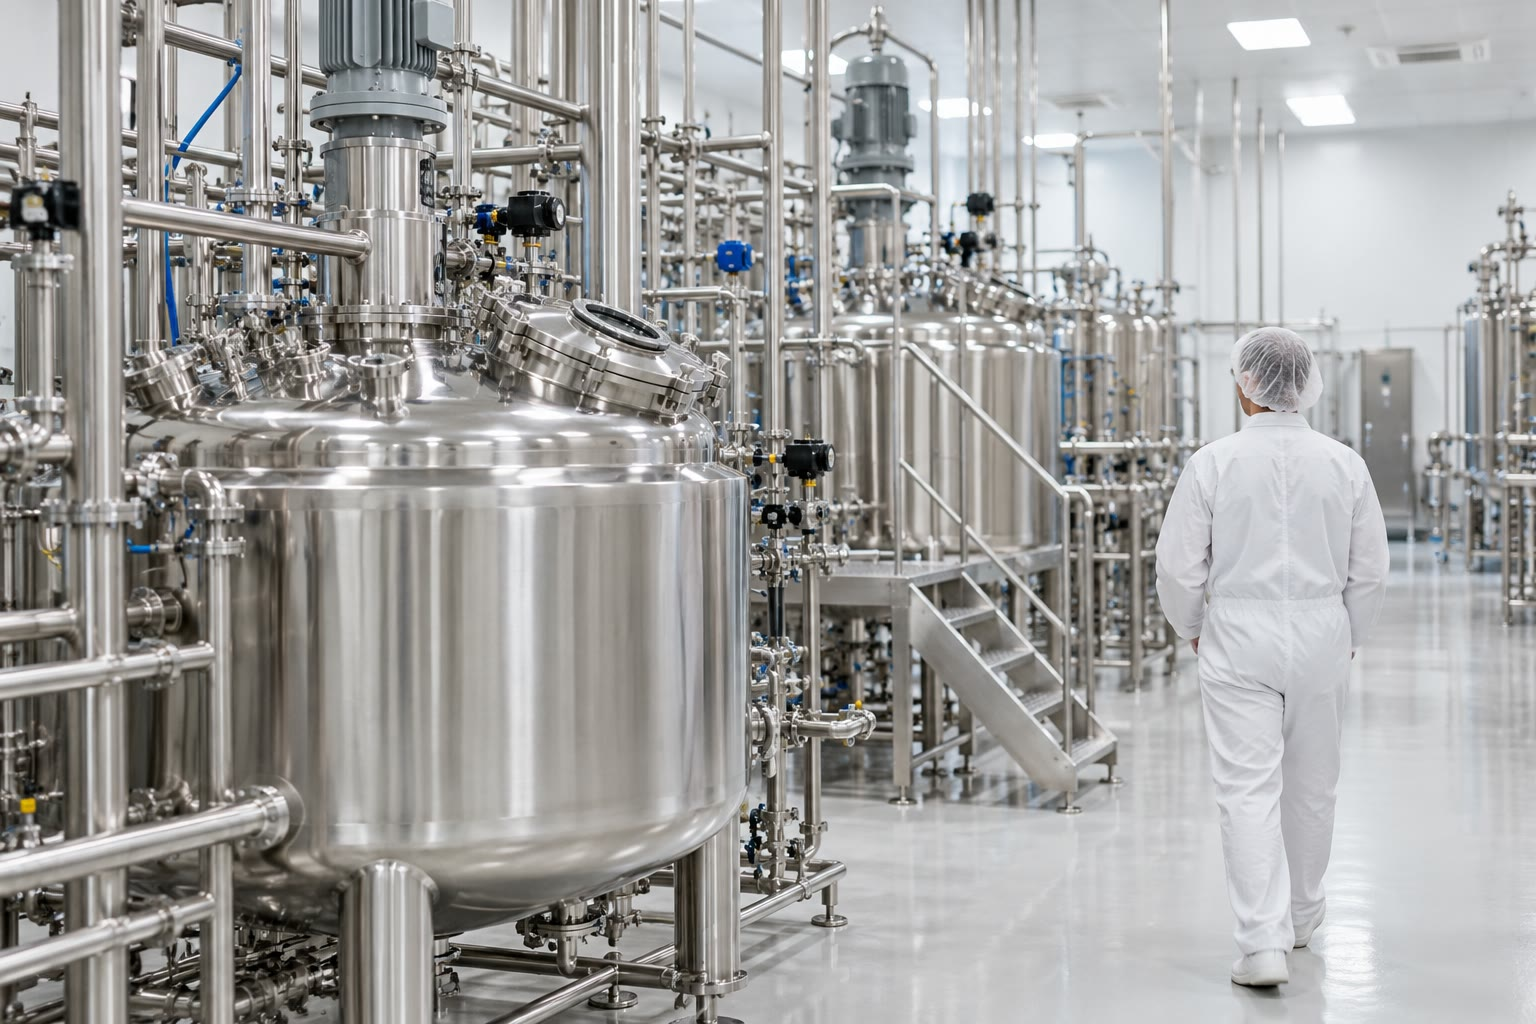
\includegraphics[width=0.48\linewidth]{images/book1/ai/g12-pharma-plant.jpg}

{\small مصنع أدوية: مفاعلات تصنيع، مكبّرة إلى
مقياس الأطنان.}
\end{omfigure}

\section{تحسين التصنيع}

يمكن تحسين أمرين مختلفين: \emph{السرعة}، التي تحدد كم
يستغرق التصنيع، و\emph{\omterm{def:g10:synthesis-yield:yield}{المردود}}، الذي يحدد كمية
\omterm{def:g7:chemical-reactions:reactant}{الناتج} التي يعطيها.

\begin{proposition}[روافع السرعة والمردود]\label{prop:g12:synthesis-strategy:levers}
\begin{itemize}
  \item تزداد السرعة بارتفاع درجة الحرارة، وبتراكيز
        \omterm{def:g7:chemical-reactions:reactant}{المتفاعلات}، وبالحفّاز.
  \item \omterm{def:g10:synthesis-yield:yield}{المردود} النهائي \omterm{def:g10:reaction-progress-table:limiting}{لتفاعل تام} يحدده \omterm{def:g7:chemical-reactions:reactant}{المتفاعل}
        المحِدّ؛ \omterm{def:g10:synthesis-yield:yield}{ومردود} \omterm{def:g12:equilibrium:non-total}{تفاعل غير تام} يزداد بفائض من
        أحد المتفاعلين، أو بنزع \omterm{def:g7:chemical-reactions:reactant}{ناتج} حالما يتكوّن. \omterm{def:g12:catalysis:catalyst}{والحفّاز}
        لا يغيّره: فهو لا يفعل إلا أن يبلغ بالمجموعة أسرع
        \omterm{def:g10:reaction-progress-table:system}{الحالة النهائية} نفسها.
\end{itemize}
\end{proposition}

\begin{proof}
النقطة الأولى تجمع العوامل الحركية في
\cref{ch:g12:reaction-rates,ch:g12:catalysis}. والثانية تنتج من
$Q = K$ في نهاية \omterm{def:g12:equilibrium:non-total}{التفاعل غير التام}: فإضافة \omterm{def:g7:chemical-reactions:reactant}{متفاعل} أو نزع
\omterm{def:g7:chemical-reactions:reactant}{ناتج} تجعل $Q < K$، فيستمر التفاعل في الاتجاه المباشر.
\end{proof}

\begin{example}[الأسترة مع مصيدة ماء]\label{ex:g12:synthesis-strategy:trap}
لا يعطي حمض الإيثانويك والإيثانول، \omterm{def:g10:the-mole:amount}{مول} من كل منهما، إلا
\qty{67}{\percent} من \omterm{def:g11:functional-groups:carboxylic-acid}{الإستر} عند التوازن. فإذا سُخّن \omterm{def:g6:pure-substances-and-mixtures:mixture}{الخليط}
بالارتداد في \omterm{def:g6:solutions-and-solubility:solute}{مذيب} لا يمتزج بالماء، مع قليل من
الحمض حفّازًا، تكاثف البخار في أنبوب جانبي، هو \emph{مصيدة
الماء}: فيستقر الماء، وهو الأكثف، في القاع ويبقى هناك، بينما
يرتد \omterm{def:g6:solutions-and-solubility:solute}{المذيب} إلى الدورق. فيغادر الماء التفاعل حالما
يتكوّن، ويبقى $Q$ أصغر من $K$، وتكاد الأسترة تبلغ
الاكتمال. فالتسخين يعطي السرعة، \omterm{def:g12:catalysis:catalyst}{والحفّاز} مزيدًا من السرعة، والمصيدة
\omterm{def:g10:synthesis-yield:yield}{المردود}.
\end{example}

\begin{omfigure}
\begin{tikzpicture}[font=\small, scale=0.8]
  \pic[transform shape] at (0,0) {hotplate};
  \pic[transform shape] at (0,0) {rbflask={0.55}{orange!20}};
  % the trap: water at the bottom, solvent above, up to the arm
  \fill[cyan!60!blue!40] (1.0,1.75) arc[start angle=180, end angle=360, radius=0.15] -- (1.3,2.3) -- (1.0,2.3) -- cycle;
  \fill[yellow!35] (1.0,2.3) rectangle (1.3,3.25);
  \draw[om glass] (-0.2,3.0) -- (-0.2,3.75) -- (0.2,3.75) -- (0.2,3.55) -- (1.0,3.55) -- (1.0,4.0);
  \draw[om glass] (0.2,3.0) -- (0.2,3.25) -- (1.0,3.25) -- (1.0,1.75) arc[start angle=180, end angle=360, radius=0.15] -- (1.3,4.0);
  \pic[transform shape] at (1.15,4.0) {condenser};
  \draw[omProp, thick, <-] (1.35,2.0) -- (2.6,1.7) node[right, text=black, align=left] {يتجمع الماء\\ في القاع};
  \draw[omProp, thick, <-] (1.35,2.9) -- (2.6,3.1) node[right, text=black, align=left] {يفيض المذيب\\ عائدًا إلى الدورق};
  \draw[omProp, thick, <-] (-0.6,0.6) -- (-1.7,1.1) node[left, text=black, align=right] {حمض، كحول،\\ حفّاز، مذيب};
\end{tikzpicture}

{\small مصيدة ماء على دورق مسخَّن بالارتداد: يُنزع الماء المتكوّن
من التفاعل حالما يتكاثف.}
\end{omfigure}

\section{الانتقائية}

كثيرًا ما يحمل \omterm{def:g7:atoms-and-molecules:molecule}{الجزيء} الحقيقي عدة مجموعات وظيفية. \omterm{def:g7:identifying-substances:characteristic-test}{والكاشف} الذي
يهاجمها كلها يعطي خليطًا؛ أما التصنيع الجيد فيستعمل كاشفًا لا يهاجم
إلا المجموعة المراد تغييرها.

\begin{definition}[التفاعل الانتقائي كيميائيًا]\label{def:g12:synthesis-strategy:chemoselective}
يكون التفاعل \emph{انتقائيًا كيميائيًا}\index{تفاعل انتقائي كيميائيًا} حين
يحوّل كاشفه، في \omterm{def:g7:atoms-and-molecules:molecule}{جزيء} يحمل عدة مجموعات وظيفية،
مجموعة واحدة ويترك الأخرى دون تغيير.
\end{definition}

\begin{example}[مختزل يختار]\label{ex:g12:synthesis-strategy:nabh4}
يختزل بوروهيدريد الصوديوم، \ce{NaBH4}، مجموعة الكربونيل في الألدهيدات
والكيتونات إلى مجموعة كحولية، لكنه لا يمس \omterm{def:g11:functional-groups:carboxylic-acid}{الإسترات}. ففي
\omterm{def:g7:atoms-and-molecules:molecule}{جزيء} يحمل \omterm{def:g11:functional-groups:carbonyl}{كيتونًا} وإسترًا، لا يتغير إلا \omterm{def:g11:functional-groups:carbonyl}{الكيتون}:
\[
  \ce{CH3-CO-CH2-CH2-CO-O-CH3}
  \;\xrightarrow{\ \ce{NaBH4}\ }\;
  \ce{CH3-CH(OH)-CH2-CH2-CO-O-CH3} .
\]
أما \omterm{def:g11:redox:oxidant}{المختزل} الأقوى، هيدريد الليثيوم والألومنيوم \ce{LiAlH4}، فكان سيختزل
المجموعتين كلتيهما: فهو ليس \omterm{def:g12:synthesis-strategy:chemoselective}{انتقائيًا كيميائيًا} هنا.
\end{example}

\begin{remark}[أنواع عدة من الانتقائية]\label{rem:g12:synthesis-strategy:kinds}
الانتقائية الكيميائية تختار بين المجموعات. ويمكن للتفاعل أيضًا أن يختار
بين موضعين للمجموعة نفسها، أو بين متماكبين فراغيين
\omterm{def:g7:chemical-reactions:reactant}{للناتج}، كما بيّنت إنزيمات \cref{ch:g12:catalysis} \omterm{def:g7:atoms-and-molecules:molecule}{والجزيئات}
الكيرالية في \cref{ch:g12:stereochemistry}. وكل نوع منها يُدرس
في المجلدات الجامعية.
\end{remark}

\section{مجموعات الحماية}

حين لا يكون أي \omterm{def:g7:identifying-substances:characteristic-test}{كاشف} انتقائيًا بما يكفي، يخفي الكيميائي المجموعة التي
يجب ألا تتفاعل، ويُجري التفاعل، ثم يكشف المجموعة من جديد.

\begin{definition}[مجموعة الحماية]\label{def:g12:synthesis-strategy:protecting-group}
\emph{مجموعة الحماية}\index{مجموعة حماية} مجموعة تُربط
\omterm{def:g11:functional-groups:functional-group}{بمجموعة وظيفية} لمنعها من التفاعل خلال خطوة أو أكثر من
التصنيع، ثم تُنزع بعد ذلك لتعيد المجموعة الأصلية.
والعمليات الثلاث هي \emph{الحماية}، و\emph{التفاعل}،
و\emph{نزع الحماية}.
\end{definition}

\begin{method}[تخطيط حماية]\label{met:g12:synthesis-strategy:plan}
\begin{enumerate}
  \item اذكر مجموعات كل \omterm{def:g7:chemical-reactions:reactant}{متفاعل}، والرابطة الوحيدة المراد تكوينها.
  \item عيّن كل مجموعة أخرى يمكن \omterm{def:g7:identifying-substances:characteristic-test}{لكاشف} تلك الخطوة أيضًا أن
        يهاجمها.
  \item احمِ كلًّا منها بمجموعة تقاوم ظروف
        التفاعل ويمكن نزعها في ظروف لطيفة
        تُبقي الرابطة الجديدة سليمة.
  \item احسب الكلفة: فكل حماية تضيف خطوتين، الحماية ونزع
        الحماية، وتخفض \omterm{def:g10:synthesis-yield:yield}{المردود} الإجمالي.
\end{enumerate}
\end{method}

\begin{example}[صنع ببتيد ثنائي واحد، لا أربعة]\label{ex:g12:synthesis-strategy:dipeptide}
يحمل كل من الغليسين والألانين مجموعة \omterm{def:g11:functional-groups:amine}{أمين} ومجموعة حمضية:
\ce{H2N-CH2-COOH} و\ce{H2N-CH(CH3)-COOH}. ورابطة \omterm{def:g11:functional-groups:amine}{أميد} بين حمض
الغليسين \omterm{def:g11:functional-groups:amine}{وأمين} الألانين تعطي الببتيد الثنائي Gly--Ala. فإذا خُلط
الحمضان الأمينيان مباشرة، أعطيا أربعة ببتيدات ثنائية، Gly--Ala وAla--Gly
وGly--Gly وAla--Ala، في \omterm{def:g6:pure-substances-and-mixtures:mixture}{خليط} يصعب فصله. والخطة:
\begin{enumerate}
  \item احمِ \omterm{def:g11:functional-groups:amine}{أمين} الغليسين بمجموعة يُرمز إليها بالرمز \ce{Z}،
        وحمض الألانين على هيئة \omterm{def:g11:functional-groups:carboxylic-acid}{إستر} الميثيل؛
  \item كوّن رابطة \omterm{def:g11:functional-groups:amine}{الأميد}: إذ لا تبقى حرة إلا مجموعة حمضية واحدة ومجموعة \omterm{def:g11:functional-groups:amine}{أمين}
        واحدة؛
  \item انزع مجموعتي الحماية كلتيهما.
\end{enumerate}
\end{example}

\begin{omfigure}
\begin{tikzpicture}[font=\small, node distance=0.55cm,
    box/.style={draw=omDef, rounded corners=2pt, fill=omDef!6, align=center, inner sep=4pt}]
  \node[box] (a) {\ce{H2N-CH2-COOH}\\ \ce{H2N-CH(CH3)-COOH}};
  \node[box, below=of a] (b) {\ce{Z-NH-CH2-COOH}\\ \ce{H2N-CH(CH3)-CO-O-CH3}};
  \node[box, below=of b] (c) {\ce{Z-NH-CH2-CO-NH-CH(CH3)-CO-O-CH3}};
  \node[box, below=of c] (d) {\ce{H2N-CH2-CO-NH-CH(CH3)-COOH}};
  \draw[->, thick, omProp] (a) -- node[right, xshift=3pt, text=black] {\foreignlanguage{arabic}{\babelsublr{1.} الحماية}} (b);
  \draw[->, thick, omProp] (b) -- node[right, xshift=3pt, text=black] {\foreignlanguage{arabic}{\babelsublr{2.} التفاعل: رابطة أميد}} (c);
  \draw[->, thick, omProp] (c) -- node[right, xshift=3pt, text=black] {\foreignlanguage{arabic}{\babelsublr{3.} نزع الحماية}} (d);
  \node[anchor=east, font=\footnotesize, text=black!70] at ([xshift=-6pt]a.west) {الغليسين، الألانين};
  \node[anchor=east, font=\footnotesize, text=black!70] at ([xshift=-6pt]d.west) {Gly--Ala};
\end{tikzpicture}

{\small الحماية، فالتفاعل، فنزع الحماية: فرابطة \omterm{def:g11:functional-groups:amine}{الأميد} الوحيدة التي يمكن أن
تتكوّن هي المطلوبة.}
\end{omfigure}

\section{الاقتصاد الذري}

\omterm{def:g10:synthesis-yield:yield}{مردود} \qty{100}{\percent} يقول إن كل \omterm{def:g7:atoms-and-molecules:molecule}{جزيء} من \omterm{def:g7:chemical-reactions:reactant}{المتفاعل}
المحِدّ صار ناتجًا. ولا يقول كم من \omterm{def:g7:atoms-and-molecules:atom}{الذرات} المشتراة
انتهى في \omterm{def:g7:chemical-reactions:reactant}{الناتج}: \omterm{def:g7:chemical-reactions:reactant}{فالنواتج} الأخرى في المعادلة، مهما كانت
نقية، نفايات ما لم يستطع أحد أن يستعملها.

\begin{definition}[الاقتصاد الذري]\label{def:g12:synthesis-strategy:atom-economy}
\emph{الاقتصاد الذري}\index{اقتصاد ذري} لتصنيع هو
نسبة كتلة \omterm{def:g7:chemical-reactions:reactant}{المتفاعلات}، مأخوذة بنسب \omterm{def:g8:balanced-equations:equation}{المعادلة
الموزونة}، التي تنتهي في \omterm{def:g7:chemical-reactions:reactant}{الناتج} المرغوب.
\end{definition}

\begin{proposition}[الاقتصاد الذري من المعادلة]\label{prop:g12:synthesis-strategy:atom-economy}
\omterm{def:g8:balanced-equations:equation}{لمعادلة موزونة} $a_1\,\ce{R1} + a_2\,\ce{R2} + \cdots \rightarrow
p\,\ce{P} + \text{نواتج أخرى}$،
\[
  \text{الاقتصاد الذري} =
  \frac{p\,M(\ce{P})}{a_1 M(\ce{R1}) + a_2 M(\ce{R2}) + \cdots}
  \times 100\,\% .
\]
\end{proposition}

\begin{proof}
لتقدم قدره $x$ \omterm{def:g10:the-mole:amount}{مول}، تكون كتلة \omterm{def:g7:chemical-reactions:reactant}{المتفاعلات} المستهلكة
$x\,(a_1 M(\ce{R1}) + \cdots)$ وكتلة \omterm{def:g7:chemical-reactions:reactant}{الناتج} المرغوب المتكوّن
$x\,p\,M(\ce{P})$؛ ونسبتهما لا تتوقف على $x$.
\end{proof}

\begin{method}[حساب الاقتصاد الذري]\label{met:g12:synthesis-strategy:atom-economy}
\begin{enumerate}
  \item اكتب \omterm{def:g8:balanced-equations:equation}{المعادلة الموزونة}؛ ولطريق من عدة خطوات، اجمع
        الخطوات بحيث يُحذف كل وسيط.
  \item احسب \omterm{def:g10:the-mole:molar-mass}{الكتلة المولية} لكل \omterm{def:g7:chemical-reactions:reactant}{متفاعل} وللناتج
        المرغوب.
  \item طبّق الصيغة، مع المعاملات الستوكيومترية.
  \item النفايات لكل كيلوغرام من \omterm{def:g7:chemical-reactions:reactant}{الناتج} هي
        $(100 - \text{الاقتصاد الذري})/\text{الاقتصاد الذري}$ كيلوغرام.
\end{enumerate}
\end{method}

\begin{example}[الإضافة مقابل الاستبدال]\label{ex:g12:synthesis-strategy:compare}
% ledger: aw:C, aw:H, aw:Br, aw:Na, aw:O
البرومو إيثان من الإيثين، \ce{C2H4 + HBr -> C2H5Br}: كل \omterm{def:g7:atoms-and-molecules:atom}{ذرة} تنتهي
في \omterm{def:g7:chemical-reactions:reactant}{الناتج}، \omterm{def:g12:synthesis-strategy:atom-economy}{والاقتصاد الذري} $108.9/(28.0 + 80.9) = \qty{100}{\percent}$.
والإيثانول من البرومو إيثان، \ce{C2H5Br + NaOH -> C2H5OH + NaBr}: اقتصاده
الذري $46.0/(108.9 + 40.0) = \qty{30.9}{\percent}$؛ أي لكل
كيلوغرام من الإيثانول، \qty{2.2}{kg} من بروميد الصوديوم. فللإضافة دائمًا
\omterm{def:g12:synthesis-strategy:atom-economy}{اقتصاد ذري} قدره \qty{100}{\percent}؛ أما \omterm{def:g12:curly-arrows:categories}{الاستبدال} أو
\omterm{def:g12:curly-arrows:categories}{الحذف} فلا يبلغه أبدًا.
\end{example}

\begin{omfigure}
\begin{tikzpicture}
\begin{axis}[width=0.8\linewidth, height=5.2cm, ybar, bar width=16pt,
    ymin=0, ymax=112, ylabel={\foreignlanguage{arabic}{الاقتصاد الذري \babelsublr{(\%)}}},
    xtick={1,2,3,4,5}, xticklabels={{الإضافة}, {الأسترة}, {\foreignlanguage{arabic}{إيبوبروفين، \babelsublr{3} خطوات}}, {\foreignlanguage{arabic}{إيبوبروفين، \babelsublr{6} خطوات}}, {الاستبدال}},
    xticklabel style={font=\footnotesize, align=center, text width=2.1cm},
    nodes near coords, nodes near coords style={font=\footnotesize},
    enlarge x limits=0.12, axis lines*=left, ymajorgrids, grid style={black!12}]
  \addplot[fill=omDef!55, draw=omDef] table[x=i, y=AE] {figdata/out/grade-12-synthesis-strategy.dat};
\end{axis}
\end{tikzpicture}

{\small اقتصادات ذرية محسوبة من المعادلات: الإيثين مع بروميد
الهيدروجين، وحمض الإيثانويك مع الإيثانول، وطريقا الإيبوبروفين،
والبرومو إيثان مع هيدروكسيد الصوديوم.}
\end{omfigure}

\section{الكيمياء الخضراء}

\begin{definition}[الكيمياء الخضراء]\label{def:g12:synthesis-strategy:green-chemistry}
\emph{الكيمياء الخضراء}\index{كيمياء خضراء} هي تصميم منتجات
وعمليات كيميائية تقلل استعمال المواد الخطرة وإنتاجها
أو تلغيهما، من اختيار المواد
الأولية إلى مصير المنتج بعد استعماله.
\end{definition}

اثنا عشر مبدأً تلخص هذا النهج؛ وكل منها سؤال يُطرح على
العملية.
% ledger: green:12
\begin{enumerate}
  \item امنع النفايات بدل معالجتها.
  \item اجعل \omterm{def:g12:synthesis-strategy:atom-economy}{الاقتصاد الذري} أكبر ما يمكن.
  \item صمّم تصنيعات أقل خطرًا.
  \item صمّم مواد كيميائية ومنتجات أكثر أمانًا.
  \item استعمل مذيبات وظروف تفاعل أكثر أمانًا.
  \item ارفع كفاءة الطاقة: اعمل قرب درجة حرارة الغرفة
        وضغطها.
  \item استعمل مواد أولية متجددة.
  \item تجنب المشتقات الكيميائية، كمجموعات الحماية.
  \item استعمل الحفّازات، لا الكواشف بكميات ستوكيومترية.
  \item صمّم منتجات تتحلل بعد استعمالها.
  \item حلّل في الزمن الحقيقي لمنع التلوث.
  \item قلّل احتمال الحوادث إلى أدنى حد.
\end{enumerate}

\begin{remark}[مبادئ لا قوانين]\label{rem:g12:synthesis-strategy:principles}
كثيرًا ما تتجاذب المبادئ في اتجاهات متعاكسة: \omterm{def:g12:synthesis-strategy:protecting-group}{فمجموعة الحماية}
تخالف المبدأ 8 لكنها قد تنقذ تصنيعًا بأكمله؛ \omterm{def:g12:catalysis:catalyst}{والحفّاز} الذي يوفر
الطاقة قد يحوي فلزًا نادرًا. والحكم على عملية يعني الموازنة بينها،
بالأرقام كلما أمكن: \omterm{def:g12:synthesis-strategy:atom-economy}{الاقتصاد الذري}، \omterm{def:g10:synthesis-yield:yield}{والمردود}، وكتلة النفايات،
والطاقة.
\end{remark}

\begin{history}[الكيمياء الخضراء، 1998]
% ledger: green:book-1998, ibu:bhc-commercial
في سنة 1998 نشر الكيميائيان بول أناستاس وجون وارنر كتابًا،
\emph{Green Chemistry: Theory and Practice}، عرض المبادئ الاثني عشر.
وقبل ذلك بسنة، كانت جائزة حكومية للتصنيعات الأكثر اخضرارًا قد
ذهبت إلى طريق الخطوات الثلاث لصنع الإيبوبروفين، المستعمل على نطاق صناعي
منذ 1992. ومنذ ذلك الحين تُدرَّس المبادئ للكيميائيين بوصفها
جزءًا من مهنتهم.
\end{history}

\begin{example}[طريقان إلى الإيبوبروفين]\label{ex:g12:synthesis-strategy:ibuprofen}
% ledger: ibu:boots-steps, ibu:bhc-steps, ibu:boots-ae, ibu:bhc-ae, ibu:bhc-ae-recovered
يُصنع الإيبوبروفين، \ce{C13H18O2}، من الهيدروكربون
\ce{C10H14} (إيزوبوتيل بنزين). ويستعمل الطريق الأقدم ست خطوات،
وفي كل منها كمية كاملة من \omterm{def:g7:identifying-substances:characteristic-test}{الكاشف}؛ ومجموع الكتل المولية لمتفاعلاته
كلها \qty{514.5}{g/mol}، مقابل \qty{206.0}{g/mol} من
الإيبوبروفين: \omterm{def:g12:synthesis-strategy:atom-economy}{فالاقتصاد الذري} \qty{40}{\percent}. ويستعمل الطريق الأحدث ثلاث
خطوات، اثنتان منها محفَّزتان، والمعادلة الإجمالية
\[
  \ce{C10H14 + C4H6O3 + H2 + CO -> C13H18O2 + C2H4O2}
\]
تعطي $206.0/266.0 = \qty{77}{\percent}$. وناتجه الثانوي، حمض الإيثانويك،
يُسترجع ويُستعمل: فإذا عُدّ ناتجًا، تجاوز \omterm{def:g12:synthesis-strategy:atom-economy}{الاقتصاد الذري}
\qty{99}{\percent}.
\end{example}

\begin{omfigure}
\chemfig{[:30]*6(-=(-[:90](-[:150])-[:30](=[:90]O)-[:-30]OH)-=-(-[:-90]-[:-150](-[:150])-[:-90])=)}

\medskip
\begin{tikzpicture}[font=\scriptsize,
    st/.style={draw=omDef, rounded corners=2pt, fill=omDef!6, minimum height=0.8cm, text width=1.15cm, align=center, inner sep=2pt}]
  \foreach \i/\t in {1/أسيلة, 2/{إضافة ذرتي كربون}, 3/ألدهيد, 4/أوكسيم, 5/نتريل, 6/حمض}
    \node[st] (o\i) at (1.7*\i,0) {\t};
  \foreach \i/\j in {1/2,2/3,3/4,4/5,5/6} \draw[->, thick] (o\i) -- (o\j);
  \node[anchor=east, align=right, font=\footnotesize] at ([xshift=-4pt]o1.west) {\foreignlanguage{arabic}{\babelsublr{6} خطوات}\\ \textbf{40 \%}};
  \foreach \i/\t in {1/أسيلة, 2/{\foreignlanguage{arabic}{إضافة \ce{H2}}}, 3/{\foreignlanguage{arabic}{إضافة \ce{CO}}}}
    \node[st, fill=omProp!8, draw=omProp] (n\i) at (1.7*\i,-1.4) {\t\\ (حفّاز)};
  \foreach \i/\j in {1/2,2/3} \draw[->, thick] (n\i) -- (n\j);
  \node[anchor=east, align=right, font=\footnotesize] at ([xshift=-4pt]n1.west) {\foreignlanguage{arabic}{\babelsublr{3} خطوات}\\ \textbf{77 \%}};
  \node[anchor=west, align=left, font=\footnotesize] at ([xshift=6pt]n3.east) {ناتج ثانوي: حمض الإيثانويك، مسترجَع؛\\ \foreignlanguage{arabic}{إذا عُدّ ناتجًا: أكثر من \babelsublr{99} \babelsublr{\%}}};
\end{tikzpicture}

{\small الإيبوبروفين (في الأعلى) وطريقا صنعه الصناعيان: الأقدم،
بست خطوات، والأحدث، بثلاث خطوات محفَّزة، مع اقتصادهما
الذري.}
\end{omfigure}

\begin{example}[مذيبات أكثر اخضرارًا]\label{ex:g12:synthesis-strategy:solvents}
% ledger: crit:CO2-T, crit:CO2-p
كثير من التفاعلات وعمليات \omterm{def:g10:chemical-species:extraction}{الاستخلاص} يستعمل مذيبات عضوية سامة أو
قابلة للاشتعال أو متطايرة. والماء أأمن المذيبات جميعًا، حين
تذوب فيه \omterm{def:g7:chemical-reactions:reactant}{المتفاعلات}. ويصير ثنائي أكسيد الكربون مذيبًا آخر: ففوق
\qty{31}{\celsius} و\qty{73.8}{bar} يكون \emph{مائعًا فوق
حرج}، لا سائلًا ولا غازًا، يذيب كثيرًا من \omterm{def:g7:atoms-and-molecules:molecule}{الجزيئات} العضوية.
وهو يستخلص الكافيين من حبوب القهوة، مثلًا؛ وحين يُخفَّض الضغط،
يعود ببساطة غازًا ولا يترك أي بقايا في
\omterm{def:g7:chemical-reactions:reactant}{الناتج}.
\end{example}

\begin{omfigure}
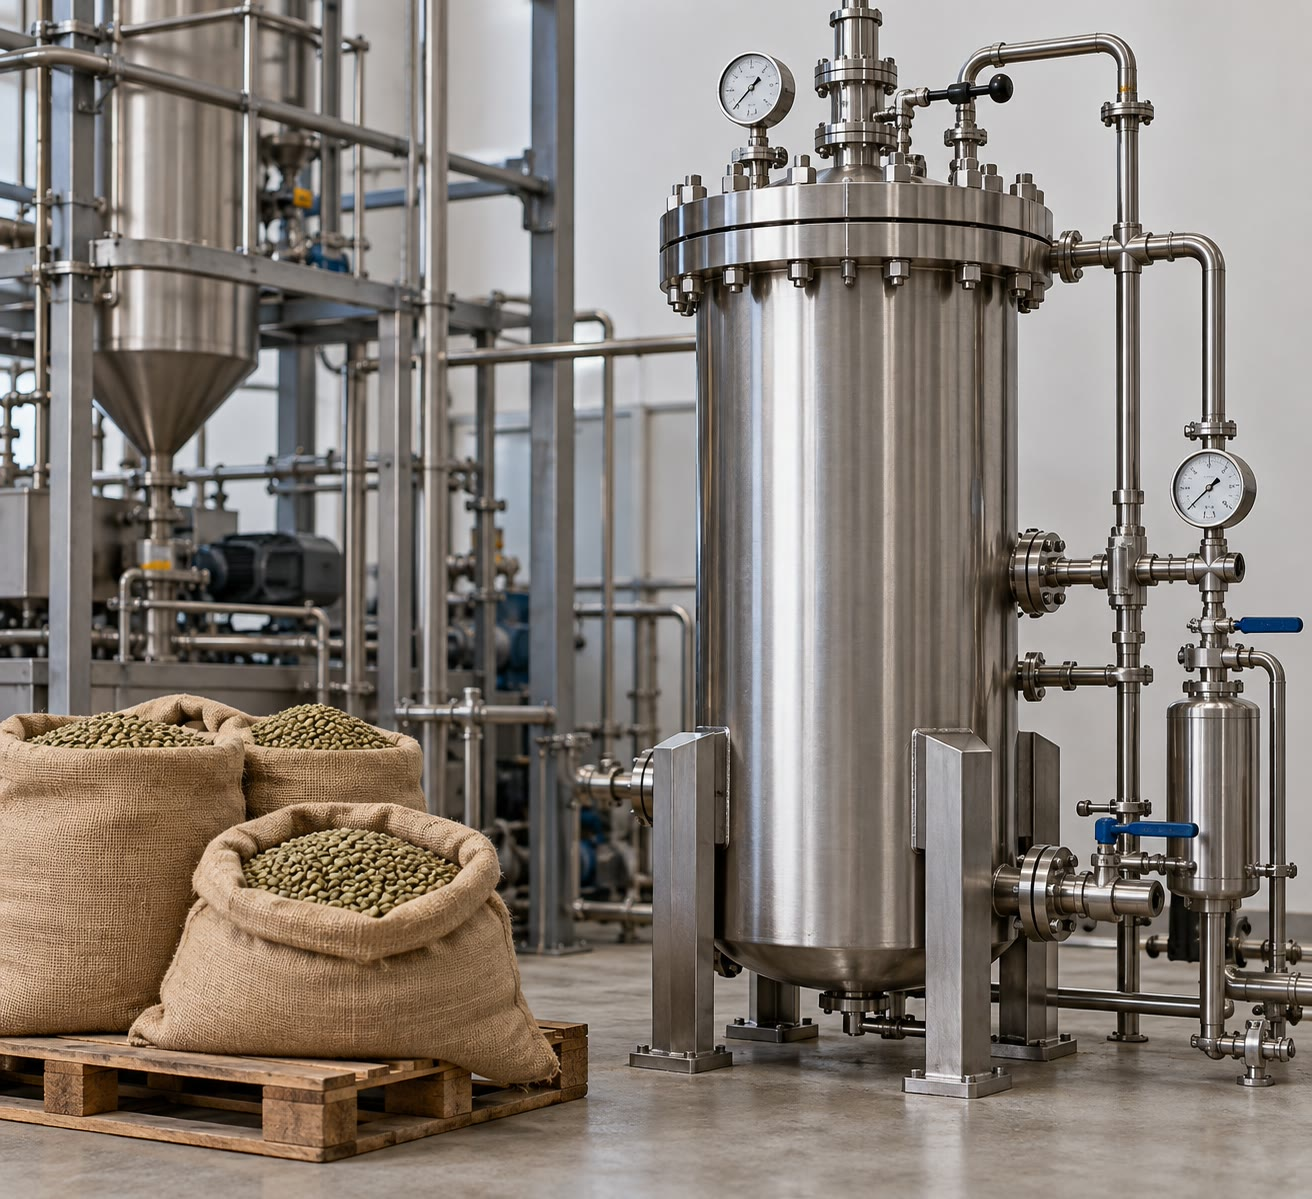
\includegraphics[width=0.45\linewidth,height=6cm,keepaspectratio]{images/book1/ai/g12-scco2-vessel.jpg}

{\small وعاء \omterm{def:g10:chemical-species:extraction}{استخلاص} عالي الضغط، يحل فيه ثنائي أكسيد الكربون فوق الحرج
محل \omterm{def:g6:solutions-and-solubility:solute}{مذيب} عضوي.}
\end{omfigure}

\section{تمارين}

\begin{exercise}[$\star$]\label{exo:g12:synthesis-strategy:1}
يمكن صنع الإيثانول بإماهة الإيثين، \ce{C2H4 + H2O -> C2H5OH}،
أو بتخمير الغلوكوز، \ce{C6H12O6 -> 2C2H5OH + 2CO2}. احسب
\omterm{def:g12:synthesis-strategy:atom-economy}{الاقتصاد الذري} لكل منهما.
\end{exercise}

\begin{exercise}[$\star$]\label{exo:g12:synthesis-strategy:2}
في مخطط الببتيد الثنائي في هذا الفصل، سمِّ الخطوة التي تُوضع فيها كل
\omterm{def:g12:synthesis-strategy:protecting-group}{مجموعة حماية}، والخطوة التي تُنزع فيها.
\end{exercise}

\begin{exercise}[$\star$]\label{exo:g12:synthesis-strategy:3}
يستبدل مصنع الماءَ \omterm{def:g6:solutions-and-solubility:solute}{بمذيب} مكلور في أحد
تفاعلاته. فأي مبدأ من مبادئ \omterm{def:g12:synthesis-strategy:green-chemistry}{الكيمياء الخضراء} يطبّق؟
\end{exercise}

\begin{exercise}[$\star$]\label{exo:g12:synthesis-strategy:4}
لماذا يرفع فائض من الإيثانول \omterm{def:g10:synthesis-yield:yield}{مردود} الأسترة، بينما
لا يرفعه \omterm{def:g12:catalysis:catalyst}{الحفّاز}؟
\end{exercise}

\begin{exercise}[$\star$]\label{exo:g12:synthesis-strategy:5}
يختزل بوروهيدريد الصوديوم الألدهيدات والكيتونات، لا \omterm{def:g11:functional-groups:carboxylic-acid}{الإسترات}. أيكون
تفاعله مع 4-أوكسو بنتانوات الميثيل (\omterm{def:g11:functional-groups:carbonyl}{كيتون} \omterm{def:g11:functional-groups:carboxylic-acid}{وإستر})
\omterm{def:g12:synthesis-strategy:chemoselective}{انتقائيًا كيميائيًا}؟ وأي مجموعة تتغير؟
\end{exercise}

\begin{exercise}[$\star\star$]\label{exo:g12:synthesis-strategy:6}
يعطي \omterm{def:g10:the-mole:amount}{مول} من حمض الإيثانويك \omterm{def:g10:the-mole:amount}{ومول} من الإيثانول \qty{0.67}{mol} من
\omterm{def:g11:functional-groups:carboxylic-acid}{الإستر} عند التوازن. اقترح طريقتين لرفع هذه الكمية، وطريقة
لبلوغها أسرع.
\end{exercise}

\begin{exercise}[$\star\star$]\label{exo:g12:synthesis-strategy:7}
يُعالَج 4-أوكسو بنتانوات الميثيل، \ce{CH3-CO-CH2-CH2-CO-O-CH3}، مرة
ببوروهيدريد الصوديوم، ومرة بفائض من هيدريد الليثيوم
والألومنيوم، الذي يختزل \omterm{def:g11:functional-groups:carboxylic-acid}{الإستر} إلى كحولين. اكتب كل \omterm{def:g7:chemical-reactions:reactant}{ناتج}.
\end{exercise}

\begin{exercise}[$\star\star$]\label{exo:g12:synthesis-strategy:8}
على المخطط الشريطي للاقتصادات الذرية، أي التفاعلات يحفظ أكثر من ثلاثة
أرباع \omterm{def:g7:atoms-and-molecules:atom}{الذرات}؟ وبأي عامل يفضل طريق الخطوات الثلاث إلى
الإيبوبروفين طريق الخطوات الست؟
\end{exercise}

\begin{exercise}[$\star\star$]\label{exo:g12:synthesis-strategy:9}
يُصنع الأسبرين بالتفاعل \ce{C7H6O3 + C4H6O3 -> C9H8O4 + C2H4O2}. احسب
اقتصاده الذري وكتلة \omterm{def:g7:chemical-reactions:reactant}{الناتج} الثانوي لكل كيلوغرام من الأسبرين.
\end{exercise}

\begin{exercise}[$\star\star$]\label{exo:g12:synthesis-strategy:10}
لماذا يُسخّن التصنيع بالارتداد لا في دورق مفتوح؟ وأيهما
يحسّن التسخين، السرعة أم \omterm{def:g10:synthesis-yield:yield}{المردود}؟
\end{exercise}

\begin{exercise}[$\star\star$]\label{exo:g12:synthesis-strategy:11}
على شكل طريقي الإيبوبروفين، عُدّ الخطوات وقل أي
مبادئ \omterm{def:g12:synthesis-strategy:green-chemistry}{الكيمياء الخضراء} يطبقها الطريق الأحدث. أعطِ ثلاثة.
\end{exercise}

\begin{exercise}[$\star\star\star$]\label{exo:g12:synthesis-strategy:12}
لتصنيع من ثلاث خطوات مردودات \qty{80}{\percent}،
و\qty{70}{\percent} و\qty{90}{\percent}. احسب \omterm{def:g10:synthesis-yield:yield}{المردود} الإجمالي.
وما كمية \omterm{def:g5:raw-materials-and-recycling:raw-material}{المادة الأولية} اللازمة للحصول على \qty{0.10}{mol} من
\omterm{def:g7:chemical-reactions:reactant}{الناتج} النهائي، إذا كان \omterm{def:g10:the-mole:amount}{المول} الواحد من \omterm{def:g5:raw-materials-and-recycling:raw-material}{المادة الأولية} يعطي في أحسن الأحوال مولًا واحدًا من
الناتج؟
\end{exercise}

\begin{exercise}[$\star\star\star$]\label{exo:g12:synthesis-strategy:13}
خطّط لتصنيع الببتيد الثنائي Ala--Gly (حمض الألانين مرتبطًا
\omterm{def:g11:functional-groups:amine}{بأمين} الغليسين): أي المجموعات تحمي، وكم خطوة
تتطلب الخطة؟
\end{exercise}

\begin{exercise}[$\star\star\star$]\label{exo:g12:synthesis-strategy:14}
تصف شركة عمليتها بأنها «خضراء» لأنها تستعمل حفّازًا. لكن
العملية تجري عند \qty{250}{\celsius} في البنزين، وهو \omterm{def:g6:solutions-and-solubility:solute}{مذيب} سام،
واقتصادها الذري \qty{35}{\percent}. احكم على هذا الادعاء، مبدأً
مبدأً.
\end{exercise}

\begin{exercise}[$\star\star\star$]\label{exo:g12:synthesis-strategy:15}
يُستخلص الكافيين من حبوب القهوة إما بثنائي كلورو الميثان، وهو
\omterm{def:g6:solutions-and-solubility:solute}{مذيب} مكلور متطاير، وإما بثنائي أكسيد الكربون فوق الحرج عند
نحو \qty{40}{\celsius} و\qty{100}{bar}. اشرح لماذا يكون الثاني
فوق حرج، ولماذا يحتاج إلى وعاء متين، وأعطِ ميزتين له
على الأول.
\end{exercise}

\section{مسألة: طريقان إلى الإيبوبروفين}

\begin{problem}[{مسألة نهاية الأسبوع --- كم من النفايات يتجنب طريق الخطوات
الثلاث لكل طن من الإيبوبروفين؟}]
\label{pb:g12:synthesis-strategy:1}
% ledger: ibu:boots-ae, ibu:bhc-ae, ibu:boots-steps, ibu:bhc-steps, aw:C, aw:H, aw:O, aw:N, aw:Cl, aw:Na
يمر الطريق الأقدم إلى الإيبوبروفين \ce{C13H18O2} بست خطوات. وإذا
جُمعت متفاعلاته كانت \ce{C10H14} و\ce{C4H6O3}
و\ce{C4H7ClO2} و\ce{C2H5ONa}، وحمض يُحسب على أنه \ce{H3O}،
و\ce{NH3O} وجزيئا \ce{H2O}. ويمر الطريق الأحدث بثلاث خطوات:
\[
  \ce{C10H14 + C4H6O3 + H2 + CO -> C13H18O2 + C2H4O2} .
\]

\medskip
\noindent\textbf{الجزء الأول --- المعادلات.}
\begin{enumerate}
  \item تحقق من أن معادلة الطريق الأحدث موزونة في الكربون
        والهيدروجين والأكسجين.
  \item سمِّ \omterm{def:g7:chemical-reactions:reactant}{الناتج} الثانوي للطريق الأحدث.
  \item في الطريق الأقدم، أي عناصر \omterm{def:g7:chemical-reactions:reactant}{المتفاعلات} تنتهي
        كلها في النفايات؟
  \item أي الطريقين يستعمل الحفّازات؟ وأي مبدأ يطبّق
        ذلك؟
\end{enumerate}

\medskip
\noindent\textbf{الجزء الثاني --- الاقتصادات الذرية.}
\begin{enumerate}[resume]
  \item احسب \omterm{def:g10:the-mole:molar-mass}{الكتلة المولية} للإيبوبروفين.
  \item احسب مجموع الكتل المولية لمتفاعلات الطريق
        الأقدم.
  \item استنتج اقتصاده الذري.
  \item احسب مجموع الكتل المولية لمتفاعلات الطريق
        الأحدث.
  \item استنتج اقتصاده الذري.
  \item كم يصير إذا عُدّ حمض الإيثانويك
        ناتجًا؟
\end{enumerate}

\medskip
\noindent\textbf{الجزء الثالث --- النفايات لكل طن.}
\begin{enumerate}[resume]
  \item للطريق الأقدم، \omterm{def:g10:synthesis-yield:yield}{بمردود} \qty{100}{\percent}، ما كتلة
        \omterm{def:g7:chemical-reactions:reactant}{المتفاعلات} المشتراة لكل طن من الإيبوبروفين؟
  \item ما كتلة النفايات التي يعطيها لكل طن؟
  \item السؤال نفسه للطريق الأحدث: كتلة \omterm{def:g7:chemical-reactions:reactant}{المتفاعلات} لكل طن.
  \item كتلة حمض الإيثانويك لكل طن.
  \item ما كتلة النفايات المتجنَّبة لكل طن إذا عُدّ حمض الإيثانويك
        من النفايات؟
\end{enumerate}

\medskip
\noindent\textbf{الجزء الرابع --- المردودات والواقع.}
\begin{enumerate}[resume]
  \item افترض أن \omterm{def:g10:synthesis-yield:yield}{مردود} كل خطوة \qty{90}{\percent}.
        احسب \omterm{def:g10:synthesis-yield:yield}{المردود} الإجمالي للطريق الأقدم.
  \item السؤال نفسه للطريق الأحدث.
  \item أعطِ سببًا آخر لكون الخطوات الأقل تعني نفايات أقل، غير
        المعادلة.
  \item في الواقع يُسترجع حمض الإيثانويك ويُستعمل. فما كتلة
        النفايات لكل طن التي يعطيها الطريق الأحدث عندئذ، \omterm{def:g10:synthesis-yield:yield}{بمردود}
        \qty{100}{\percent}؟
  \item اذكر الجواب النهائي: كم من النفايات يتجنب طريق الخطوات الثلاث
        لكل طن من الإيبوبروفين؟
\end{enumerate}
\end{problem}
